\documentclass[a4paper,10pt,twoside]{article}
\usepackage[utf8]{inputenc}
\usepackage[french]{babel}
\usepackage[T1]{fontenc}
\usepackage{amsmath}
\usepackage{amsfonts}
\usepackage{amssymb}
\usepackage{graphicx}
\usepackage{multicol}
\usepackage{array}
\usepackage{float}
\usepackage{epstopdf}
\usepackage[justification=centering]{caption}
\usepackage{caption}
\usepackage{subfig}
\usepackage{gensymb}
\usepackage[bottom]{footmisc}
\usepackage{appendix}
\usepackage{pdfpages}
\usepackage{todonotes}
\usepackage{mathpazo}
\usepackage{titleps}
\usepackage{color}
\usepackage{hyperref}
\usepackage[skins]{tcolorbox}
\usepackage{sectsty}
\usepackage[arrowmos]{circuitikz}
\usepackage{blindtext}
\usepackage{adjustbox}
\usepackage{listings}
\usepackage[inner=2.5cm,outer=2.5cm,top=3cm,bottom=3cm]{geometry}

\graphicspath{{pictures/}}
\setlength\parindent{0pt}
\renewcommand*\rmdefault{ppl}
\newcolumntype{C}[1]{>{\centering\let\newline\\\arraybackslash\hspace{0pt}}m{#1}}
\newcolumntype{R}[1]{>{\raggedright\arraybackslash}p{#1}}
\sectionfont{\large}
\subsectionfont{\normalsize}

% Page style definitions
\newpagestyle{main}{
	\sethead[Club ELEC : Hands-on 3][][]  % even
			{\chaptertitle}{}{Club ELEC : Hands-on 3}
	\headrule
    \setfoot[\thepage][][]
    		{}{}{\thepage}
}

\newpagestyle{appendix}{
	\sethead[Club ELEC : Annexes][][]  % even
			{}{}{Club ELEC : Annexes}
	\headrule
    \setfoot[\thepage][][]
    		{}{}{\thepage}
    \footrule
}

%----------------------------------------------------------------------------------------
%	TITLE SECTION
%----------------------------------------------------------------------------------------
\title{
	\vspace{2.5cm}
	\normalfont \normalsize
	\huge Club ELEC\\
	\vspace{2.5cm}
	\huge Projet Robot\\
	\vspace{.25cm}
	\Large HO3 - Détection de ligne
	\vspace{2.5cm}
	\centering
}

\begin{document}
\renewcommand{\figurename}{Fig.}
\renewcommand{\thepage}{\roman{page}}
\setcounter{page}{1}

\pagenumbering{gobble}
\maketitle
\newpage
\pagenumbering{arabic}
\pagestyle{main}

\newpage
\null
\thispagestyle{empty}
\newpage
\clearpage

\setcounter{page}{1}

%%% Introduction
\section*{Introduction}
\section{Introduction}

Grâce au HO2, vous avez été réussi à transformer un signal sonore en un signal carré en utilisant principalement un compareteur, un diviseur résistif et un NE555. L'allure de ces signaux est présentée à la Figure~\ref{fig:signal-all}. En principe, votre circuit fonctionne donc comme attendu, bien joué !

\begin{figure}[h!]
    \centering
    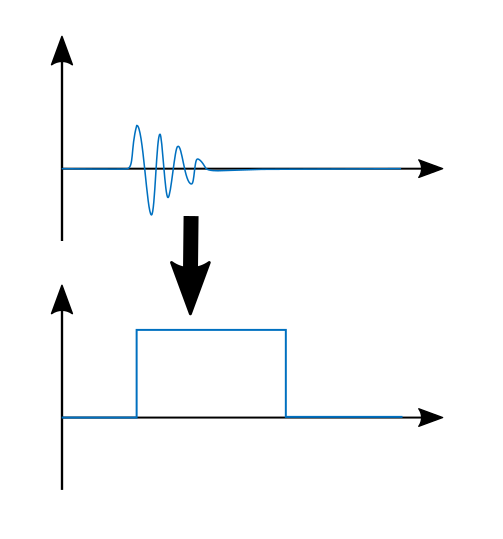
\includegraphics[width=0.5\textwidth]{signals.PNG}
    \caption{Transformation du signal HO2}
    \label{fig:signal-all}
\end{figure}

Maintenant, il va falloir utiliser ce signal carré pour générer le signal de commande: celui-ci doit passer de 0[V] à 5[V] ou de 5[V] à 0[V] lorsqu'un signal carré est généré par un évènement sonore. Vous devez donc reproduire le signal de la Figure~\ref{fig:signal-all_HO3}. Cela vous permettra \textit{in fine} d'utiliser un interrupteur (transitor) connecté à une LED afin de l'allumer ou l'éteindre. Le signal orange à la Figure~\ref{fig:signal-all_HO3} est donc bel et bien votre \textbf{signal de commande}. \\

\begin{figure}[h!]
    \centering
    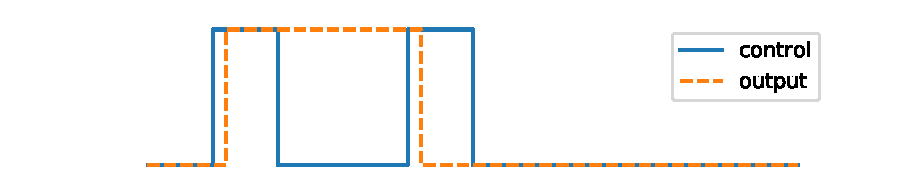
\includegraphics[width=1\textwidth]{figures/signals_control.pdf}
    \caption{Transformation du signal HO3}
    \label{fig:signal-all_HO3}
\end{figure}

%%% Objectifs du HO1
\section*{Objectifs}
% Objectifs: prise en main du micro et du signal sonore, notion AC/DC, utilisation de l'oscilloscope, découplage AC

Les objectifs du premier hands-on sont:

\begin{itemize}
	\item[-] De se familiariser avec le matérial de base (breadboard, multimètre, oscilloscope) et les composants de base (résistances, capacités, amplificateurs opérationnels, composants intégrés) propres à l'électronique.
	\item[-] De comprendre le fonctionnement du micro qui assure la transduction du signal sonore en signal électrique.
	\item[-] De faire le lien entre le signal obtenu et son contenu fréquentiel afin de comprendre la notion de filtrage.
	\item[-] De comprendre la notion AC/DC et le découplage AC.
	\item[-] D'implémenter en pratique la première partie du circuit (micro, filtre et découplage).
\end{itemize}

\begin{figure}[!ht]
	\centering
	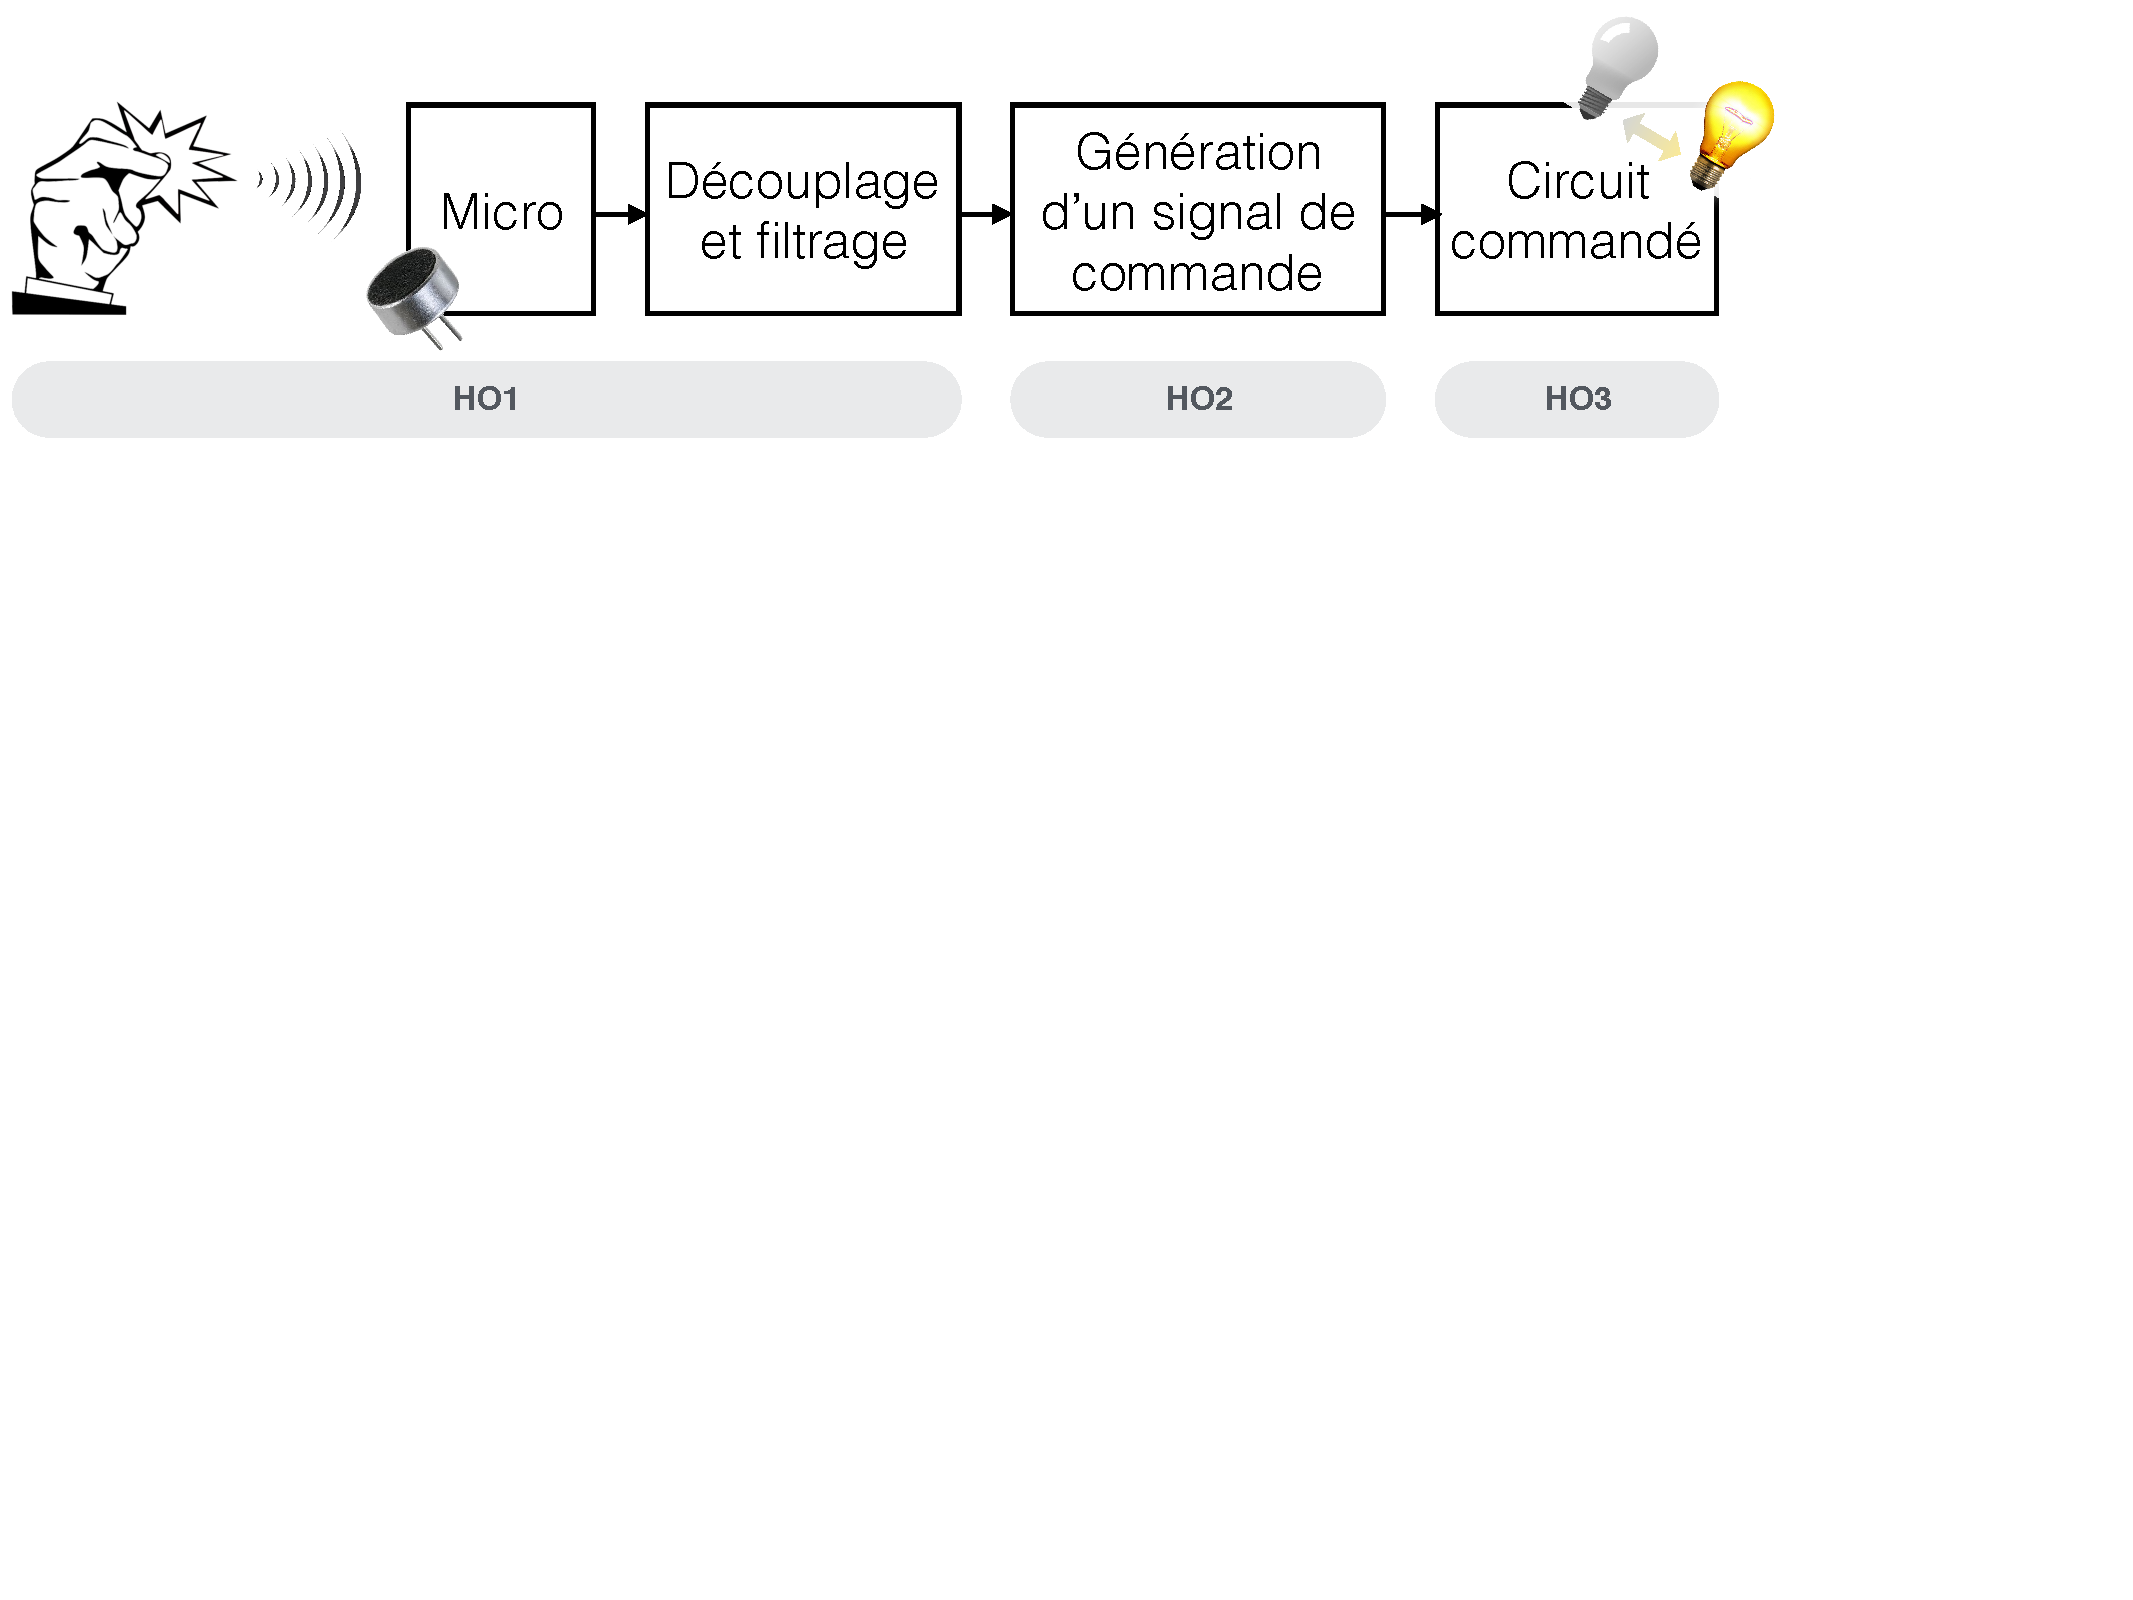
\includegraphics[width=.75\textwidth]{figures/SchemaBloc.pdf}
	\caption{Schéma-bloc du circuit.}
	\label{fig:block-diagram}
\end{figure}

Le schéma-bloc du circuit est présenté à la Figure \ref{fig:block-diagram}. Les ondes acoustiques générées par le claquement de doigt sont captées par le micro qui les transforme en un signal électrique (transduction). Ce signal est ensuite découplé et filtré à l'aide d'un filtre RC, comme présenté plus loin dans ce document. La génération d'un signal de commande propre ainsi que l'implémentation d'un circuit commandé seront abordées plus en détail dans les prochain hands-on.


%%% Assemblage du robot
\section*{Connexion des blocs}
Pour la connexion des différentes parties découvertes lors des dernières séances, vous devriez être maintenant capables de vous en sortir avec les informations déjà reçues. Si vous avez la moindre question, les membres du Club se feront un plaisir de vous aider!\\

Jusqu'ici, vos circuits étaient alimentés par une tension de 5V, provenant soit d'une source fixe ou soit d'un câble USB. Pour rendre votre robot autonome dans ses déplacements, vous recevrez une pile 9V ainsi qu'un connecteur. Connectez les masses ensemble et la tension positive de la pile (fil rouge du connecteur) au port VIN de l'Arduino. Ce port permet de recevoir une tension d'alimentation entre 7V et 12V, qui est réduite à 5V par un régulateur interne de l'Arduino. Cette tension de 5V est utilisée par l'Arduino pour fonctionner et peut également être utilisée pour alimenter des circuits externes (par exemple le récepteur infrarouge) grâce à la sortie 5V. Comme le moteur consomme beaucoup de puissance, pour éviter de surcharger le régulateur de tension de l'Arduino, ne branchez pas l'alimentation $V_{DD,moteur}$ (cfr. hands-on 1) sur le 5V mais directement sur le 9V de la pile. Cela permettra également au moteur de tourner plus vite. ATTENTION! Ne branchez pas le 9V sur $V_{DD,controle}$, qui reste branché sur le 5V.\\



\section*{Assemblage du robot}
Maintenant que vous avez bien compris le fonctionnement d'un moteur DC et du pont H qui permet de le contrôler, il est temps de passer à la pratique! Durant ce premier hands-on, vous allez pouvoir connecter votre premier moteur DC ainsi que de le contrôler à l'aide des signaux électriques.\\

Dans la section précédente, vous avez pu vous familiariser avec le schéma d'un pont H. Ce circuit peut être réalisé soit à partir de composants discrets séparés, typiquement dans des applications nécessitant de hautes puissances et donc des composants plus conséquents, mais il existe également des versions intégrées dans des puces électroniques prêtes à l'emploi. Utilisées essentiellement dans des petites applications lorsque les courants et tensions ne sont pas trop élevés, celles-ci offrent un gain en taille et en coût qui permet de réaliser un petit circuit de contrôle assez facilement. C'est cette seconde approche que nous utiliserons dans ce projet, à l'aide du composant L293D de Texas Instruments.\\

Le L293D comprend 4 demi-ponts H, comme vous pouvez le voir à la Figure~\ref{L293}. Ces demi-ponts peuvent être utilisés soit séparément, soit par 2 pour former le pont H tel que vous l'avez vu dans la section précédente. Quelques petites observations intéressantes sur ce schéma:
\begin{itemize}
\item Un signal de contrôle supplémentaire (EN) permet de déconnecter la borne Y de son circuit de contrôle.
\item Le L293 nécessite 2 alimentations séparées: une pour le contrôle des interrupteurs et une pour alimenter le pont H (et donc le circuit connecté à sa sortie). Cette séparation est très pratique, par exemple pour contrôler des moteurs qui nécessitent une tension élevée (9V dans notre cas), à l'aide de signaux provenant d'un microcontrôleur (typiquement 5V). Dans ce premier hands-on, pour la simplicité, les 2 alimentations seront connectées à 5V.
\item La masse du circuit est connectée à 4 broches du boîtier. Cela permet non seulement d'assurer une bonne conductivité, mais aussi de dégager la chaleur générée par les forts courants qui peuvent apparaître dans la puce. Cette chaleur est alors redistribuée dans la breadboard ou le PCB.\\
\end{itemize}

\begin{figure}[!t]
\centering
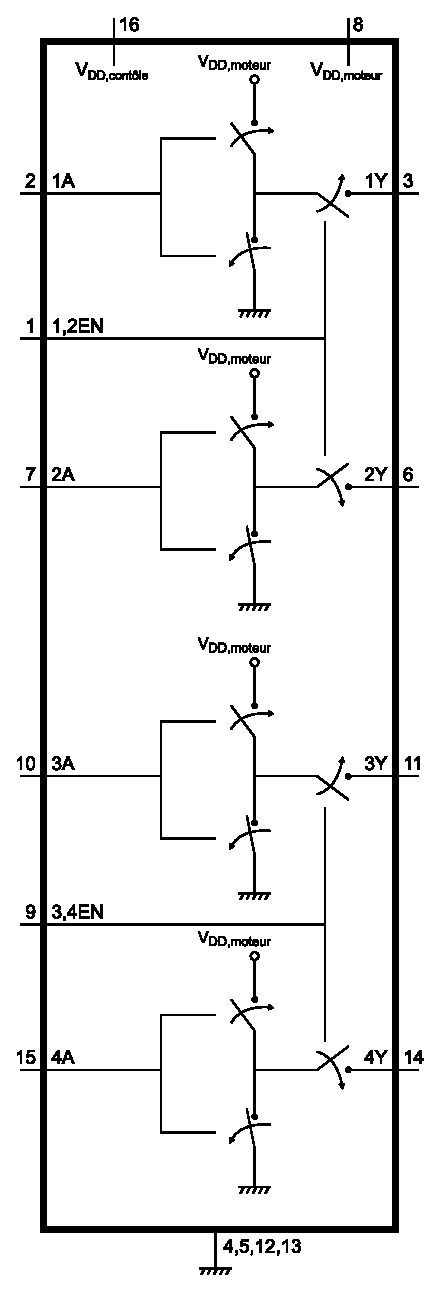
\includegraphics{L293.eps}
\caption{Schéma simplifié du L293D. Les numéros indiqués près des entrées/sorties correspondent aux numéros des broches de la puce.}
\label{L293}
\end{figure}


Vous pouvez maintenant réaliser sur une breadboard le petit circuit de contrôle illustré à la Figure~\ref{circuit}. Ce circuit utilise 2 demi-ponts H du L293. ATTENTION à ne pas oublier les diodes et à les connecter dans le bon sens. Comme expliqué précédemment, si ces diodes ne sont pas connectées correctement, le courant qui apparait lors de la décharge de l'énergie magnétique risquerait d'endommager le L293. N'hésitez pas à demander à l'un des membres du Club Elec de vérifier votre circuit si vous avez le moindre doute!\\

\begin{figure}[!t]
\centering
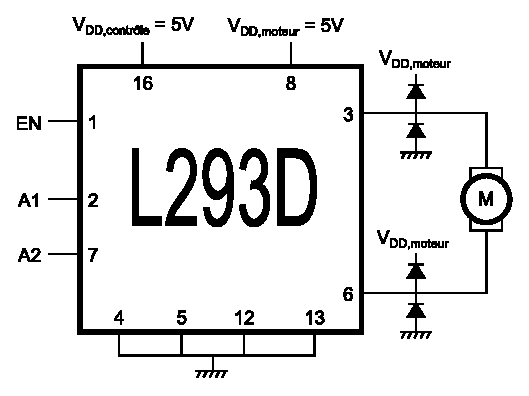
\includegraphics{circuit.eps}
\caption{Contrôle d'un moteur à l'aide du L293D. Les broches non indiquées sur le schéma peuvent être laissées flottantes ou connectées à la masse.}
\label{circuit}
\end{figure}

Essayez maintenant de connecter les signaux de contrôle (EN, A1, A2) à l'alimentation de 5V ou à la masse. Qu'observez-vous sur le moteur? Cela correspond-t-il bien à ce à quoi vous vous attendiez? Vérifiez avec le comportement attendu repris dans la Table~\ref{signal}.\\

\begin{table}[!t]
\caption{Signaux de contrôle pour le moteur DC}
\begin{center}
\begin{tabular}{|l|l|l|l|}
\hline
\textbf{EN}& \textbf{A1} & \textbf{A2} &\textbf{Moteur}\\
\hline
5V & 0V & 5V & Tourne dans un sens\\
5V & 5V & 0V & Tourne dans l'autre sens\\
5V & 0V & 0V & Freine\\
5V & 5V & 5V & Freine\\
0V & X & X & Libre\\
\hline
\end{tabular}
\label{signal}
\end{center}
\end{table}

S'il vous reste du temps, connectez l'entrée EN à un générateur de signal et générez un signal rectangulaire entre 0 et 5V. Que se passe-t-il lorsque vous faites varier le duty-cycle (rapport du temps à 5V et à 0V) de ce signal.


%%% Détection de ligne
\section*{Détection de ligne}
Une partie du concours sera réservée aux robots capables de suivre une ligne tracée au sol, indépendamment de tout contrôle humain. Si vous désirez y participer, vous trouverez ci-dessous les instructions pour la connexion du capteur et la programmation de l'Arduino. \\

Comme illustré à la Figure~\ref{fig:circuit}, la détection d'une ligne se fait à partir d'une LED et d'une photodiode. Le principe de base du fonctionnement est assez simple: la LED éclaire une surface et la photodiode mesure la partie de la lumière qui est réfléchie. En fonction de la couleur de la surface, plus ou moins de lumière sera réfléchie, ce qui permet donc de déterminer si on est au-dessus d'une ligne noire ou au-dessus d'une surface blache à partir de la mesure de la photodiode.\\

La façon dont le circuit de lecture de la photodiode fonctionne est un peu plus subtile. Les plus attentifs auront peut-être remarqué que la diode semble être branchée à l'envers, dans le sens non-passant avec la cathode du côté positif et l'anode du côté négatif. Du coup, comment fait-on pour effectuer une mesure si aucun courant ne passe? En réalité, quand une diode est branchée dans le sens non-passant, un courant très faible passe néanmoins. Dans une photodiode, ce courant va dépendre de la quantité de lumière reçue dans un certain intervalle de longueurs d'ondes (dans notre cas pour des lumières infrarouges). Ce courant qui varie, de l'ordre de quelques nA dans le noir à plusieurs $\mu$A à la lumière, passe à travers une résistance, ce qui crée donc une variation de la différence de potentiel. En lisant la tension grâce à l'ADC de l'Arduino sur la broche A0, on peut donc détecter un changement de lumière.\\

\begin{figure}[!t]
\centering
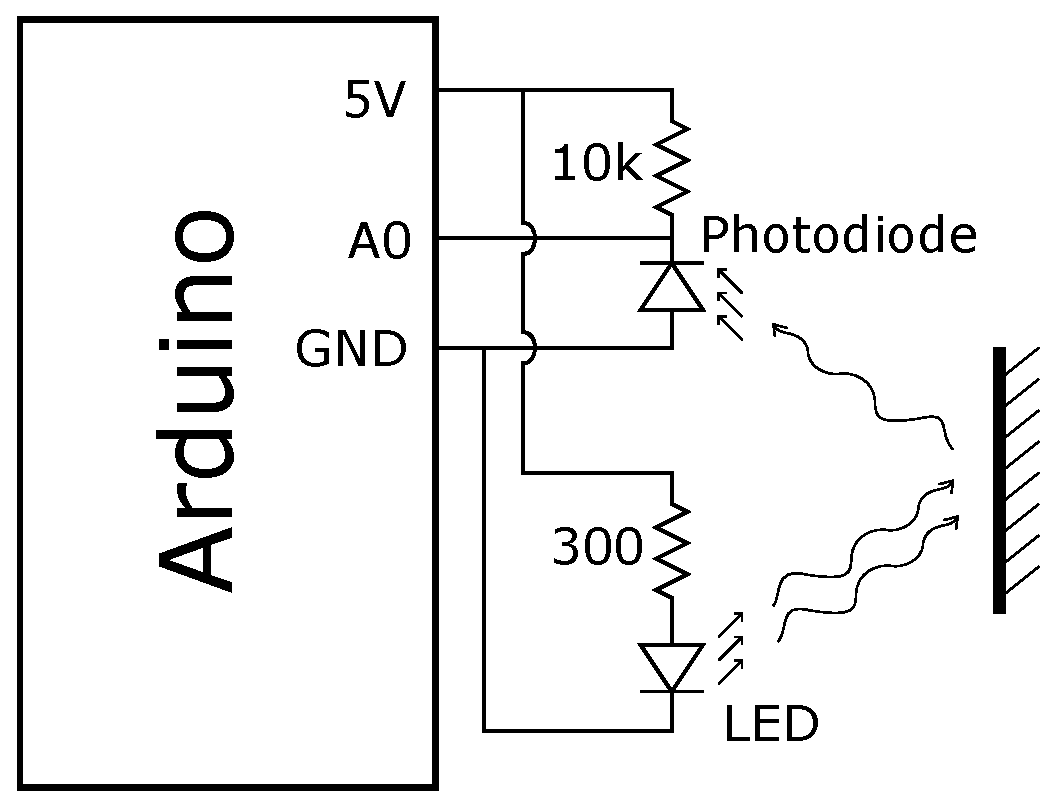
\includegraphics[width=0.4\textwidth]{imgs/circuit.eps}
\caption{Circuit et principe de fonctionnement pour la détection de ligne.}
\label{fig:circuit}
\end{figure}

Dans le code, la lecture de la tension se fait grâce à la fonction \textit{analogRead(pin)}. Vous pouvez faire l'essai avec le morceau de code ci-dessous. Observez le changement de ce qui s'affiche dans le terminal en fonction de la surface qui fait face au capteur. 

\lstset{language=C}
\begin{lstlisting}[frame=single,numbers=left,numberstyle=\small,label={code1},caption={Lecture de la photodiode.}]
const int PHOTO_PIN = 14;

int val = 0; 

void setup() {
  Serial.begin(9600); 
}

void loop() {
  val = analogRead(analogPin);  
  Serial.println(val);      
  delay(300);
}

\end{lstlisting}

A partir de cette valeur, vous pouvez maintenant essayer de programmer le contrôle du mouvement de votre robot. Il existe énormément de stratégies possibles, des très simples aux plus compliquées, avec un ou plusieurs capteurs. A vous de réfléchir à ce que votre robot doit viser comme valeur sur les capteurs, quand et comment tourner pour rester le plus proche possible de la ligne... Pour vous aider, n'hésitez pas à aller faire un tour sur Internet, certains projets en ligne pourront probablement vous aider!

\end{document}
